\documentclass[11pt,a4wide]{article}
\usepackage{verbatim}
\usepackage{listings}
\usepackage[pdftex]{graphicx}
\usepackage{a4wide}
\usepackage{color}
\usepackage{amsmath}
\usepackage{amssymb}
\usepackage[dvips]{epsfig}
\usepackage[T1]{fontenc}
\usepackage{cite} % [2,3,4] --> [2--4]
\usepackage{shadow}
\usepackage{hyperref}

\setcounter{tocdepth}{2}

\lstset{language=c++}
\lstset{basicstyle=\small}
\lstset{backgroundcolor=\color{white}}
\lstset{frame=single}
\lstset{stringstyle=\ttfamily}
\lstset{keywordstyle=\color{red}\bfseries}
\lstset{commentstyle=\itshape\color{blue}}
\lstset{showspaces=false}
\lstset{showstringspaces=false}
\lstset{showtabs=false}
\lstset{breaklines}
\begin{document}
\section*{Project 3}
\section*{Evan Markel}

My C++ program is located here in GitHub \url{https://github.com/evanmarkel/Project3}

\section*{Introduction}
%
In this project, I have used numerical methods to solve second order differential equations to simulate the solar system. Using relative units for distance, velocity, and mass, I was able to discretize the equations in unitless quantities similar to previous projects. The Runge-Kutta4 method and Verlet algorithm have proven very accurate in modeling celestial dynamics according to Newton's and Kepler's laws. We begin by separating Newton's second law of motion into into its two-dimensional Cartesian components for a circular orbit here: 
\[
\frac{d^2x}{dt^2}=\frac{F_{G,x}}{M_{\mathrm{Earth}}},
\]
and 
\[
\frac{d^2y}{dt^2}=\frac{F_{G,y}}{M_{\mathrm{Earth}}},
\]\newline
We then can use these equations along with the equation for force below to derive four coupled first order differential equations for celestial motion in two-dimensions. 
\[
F_G= \frac{M_{\mathrm{body1}}v_{body1}^2}{r}=\frac{GM_{body2}M_{\mathrm{body1}}}{r^2},
\]\newline
We then express the motion of body 1 around body 2 with four component time derivatives: 
\[
\frac{dv_{x1}}{dt}=\frac{-G*M_{body2}}{r^{3}}*x_{body1}, \hspace{.5 cm} \frac{dx_{body1}}{dt}=vx_{body1}
\]
and
\[
\frac{dv_{y1}}{dt}=\frac{-G*M_{body2}}{r^{3}}*y_{body1}, \hspace{.5 cm} \frac{dy_{body1}}{dt}=vy_{body1}
\]
The above equations now become the and utilizing the numerical Verlet, Euler-Cromer, and Runge-Kutta algorithms to solve the differential equations pertaining to the time derivatives in the physical laws. 

\newpage
\begin{enumerate}
\item[\bf Two-Body Problem]
These equations nicely predict the motion of the earth around the sun in my simulation. My code creates a celestial object which generates a vector in the SolarSystem class that contains the initial position and velocity for the object in two dimensions. The system is then updated using the RK4 method and the new position and velocity are logged. Proceeding in this manner, the plot of these data points produces the orbit. This graph runs for 100 years with a calculation step length of .01 years. The broad blue band shows the oscillation in the orbit.  For the Earth, we can easily find the needed initial velocity for circular motion: 
\[
v_{earth}^2r=GM_{\odot}=4\pi^2\mathrm{AU}^3/\mathrm{yr}^2.
\]\newline
For $r=1AU$ we see that in these units $v_{earth}=2*\pi$. Using this velocity and initial position of (1AU,0) we get a stable orbit. 
\begin{figure}
\centering
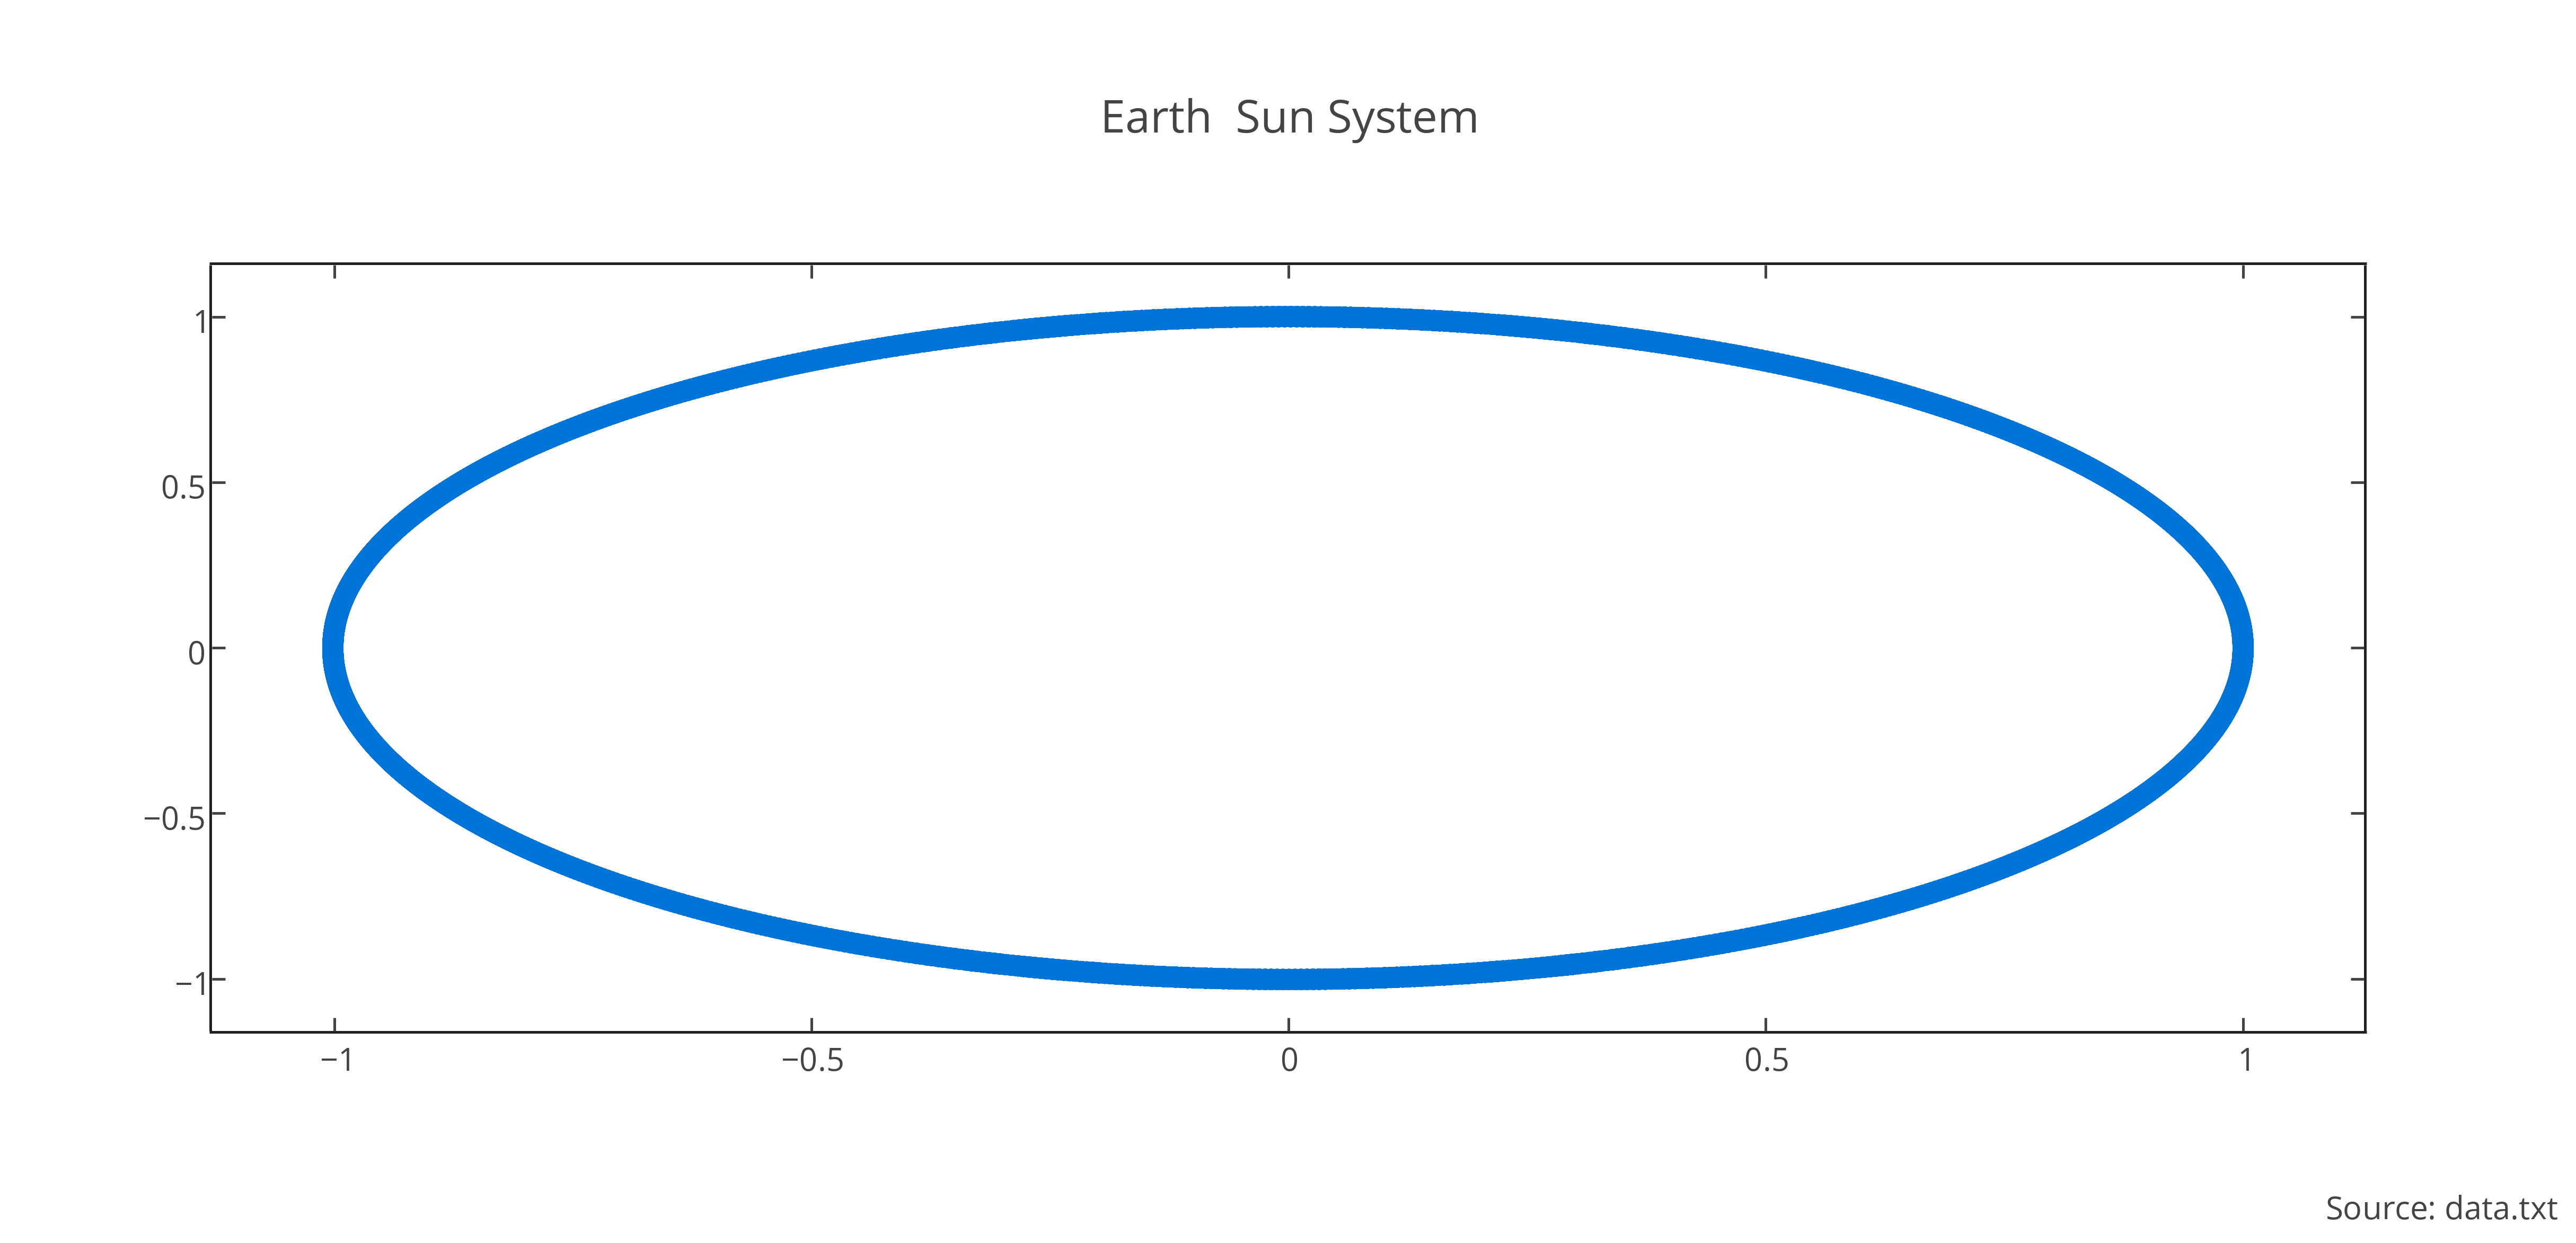
\includegraphics[width=6in, height=6in]{earth_sun_system.png}\\
\end{figure}
This orbit is stable as we can see from the graph. Earth orbits the sun (invisible at center). The mass of earth is given in the relative units of the sun's mass (3e-6) and the distance is 1AU. Also, the kinetic energy, potential energy, and angular momentum are all constant in this simple scenario. We see that $KE=\frac{1}{2}*m*v^{2}$, $PE=\frac{M_{\odot}*M_{earth}}{distance=1AU}$, and $L=distance x velocity$ are constant with constant velocity, distance. In this scenario I found the kinetic energy to be 5.9217e-5 and the potential energy to be the mass of the earth in the given units ($M_{\odot}$ and $r$ = 1). 
Changing the velocity of Earth can disrupt this stable orbit. I found that by increasing the velocity by about 40 percent will allow the earth to escape the sun's gravity. There is an analytical solution as the escape velocity is given by
\[
\it v_{escape}=\sqrt{\frac{2*G*M_{\odot}}{r}}
\] We can see that at $v_{earth} = \sqrt{8}*\pi$ earth does escape. In more physical units, the escape velocity of Earth is 42.1 km/s. 
\centering
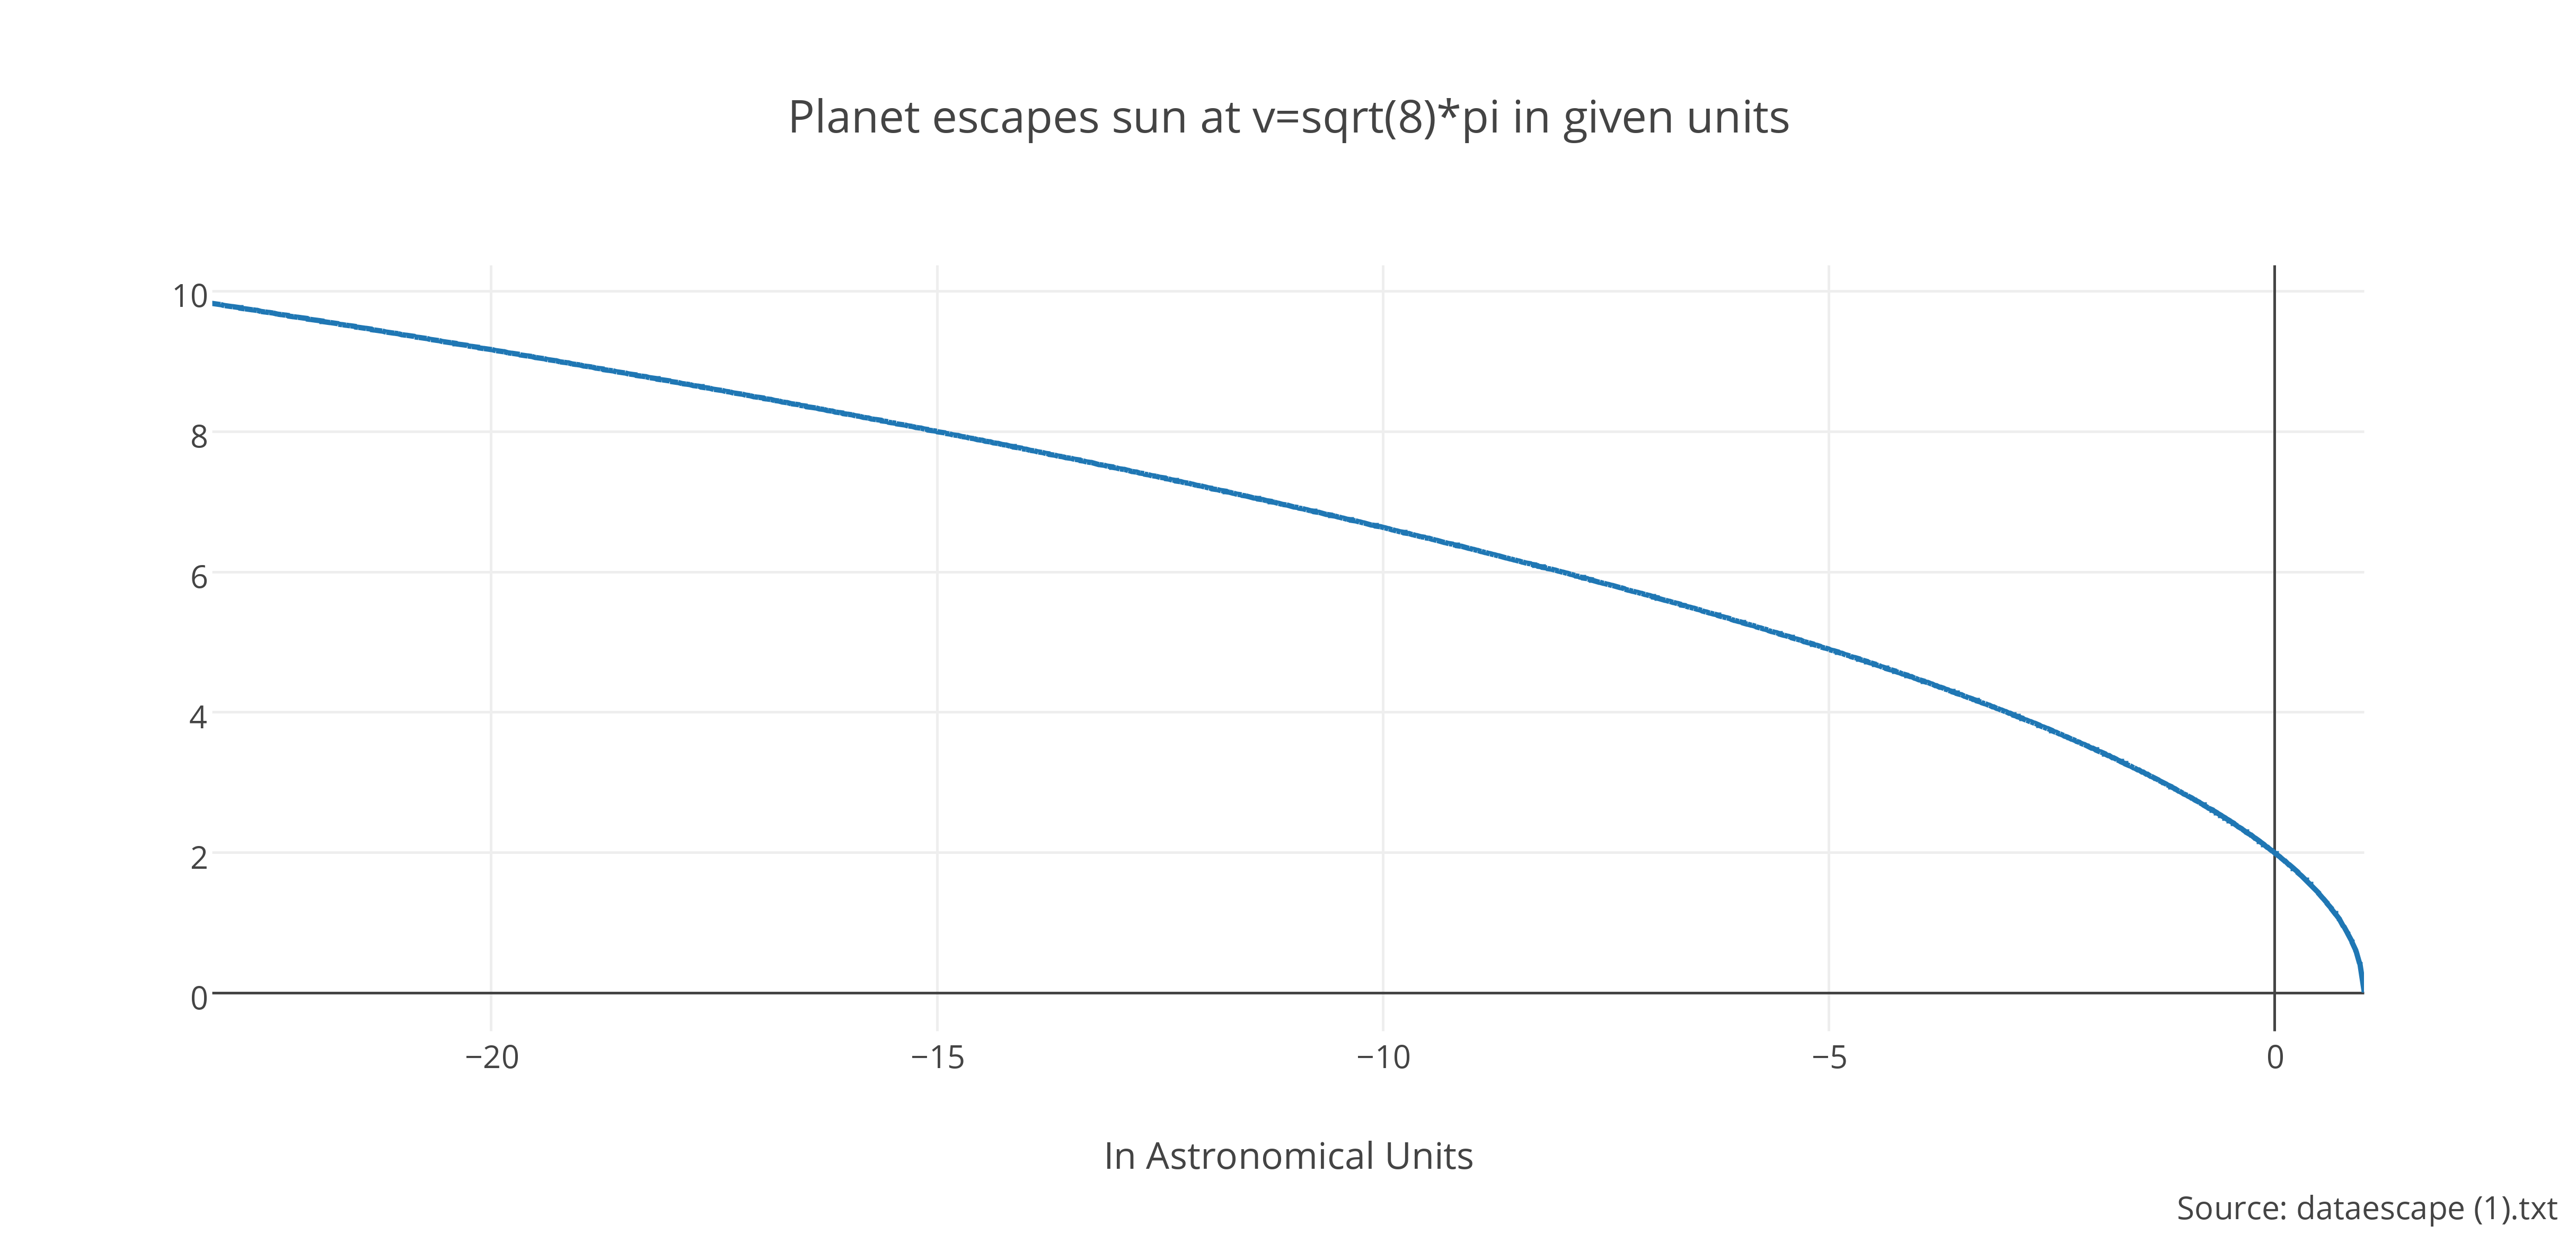
\includegraphics[width=6in]{planet_escapes_sun_at_vsqrt8pi_in_given_units.png}\\
However, at $v_{earth} = \sqrt{7.5}*\pi$, the earth does not escape but instead takes a much longer orbit. 
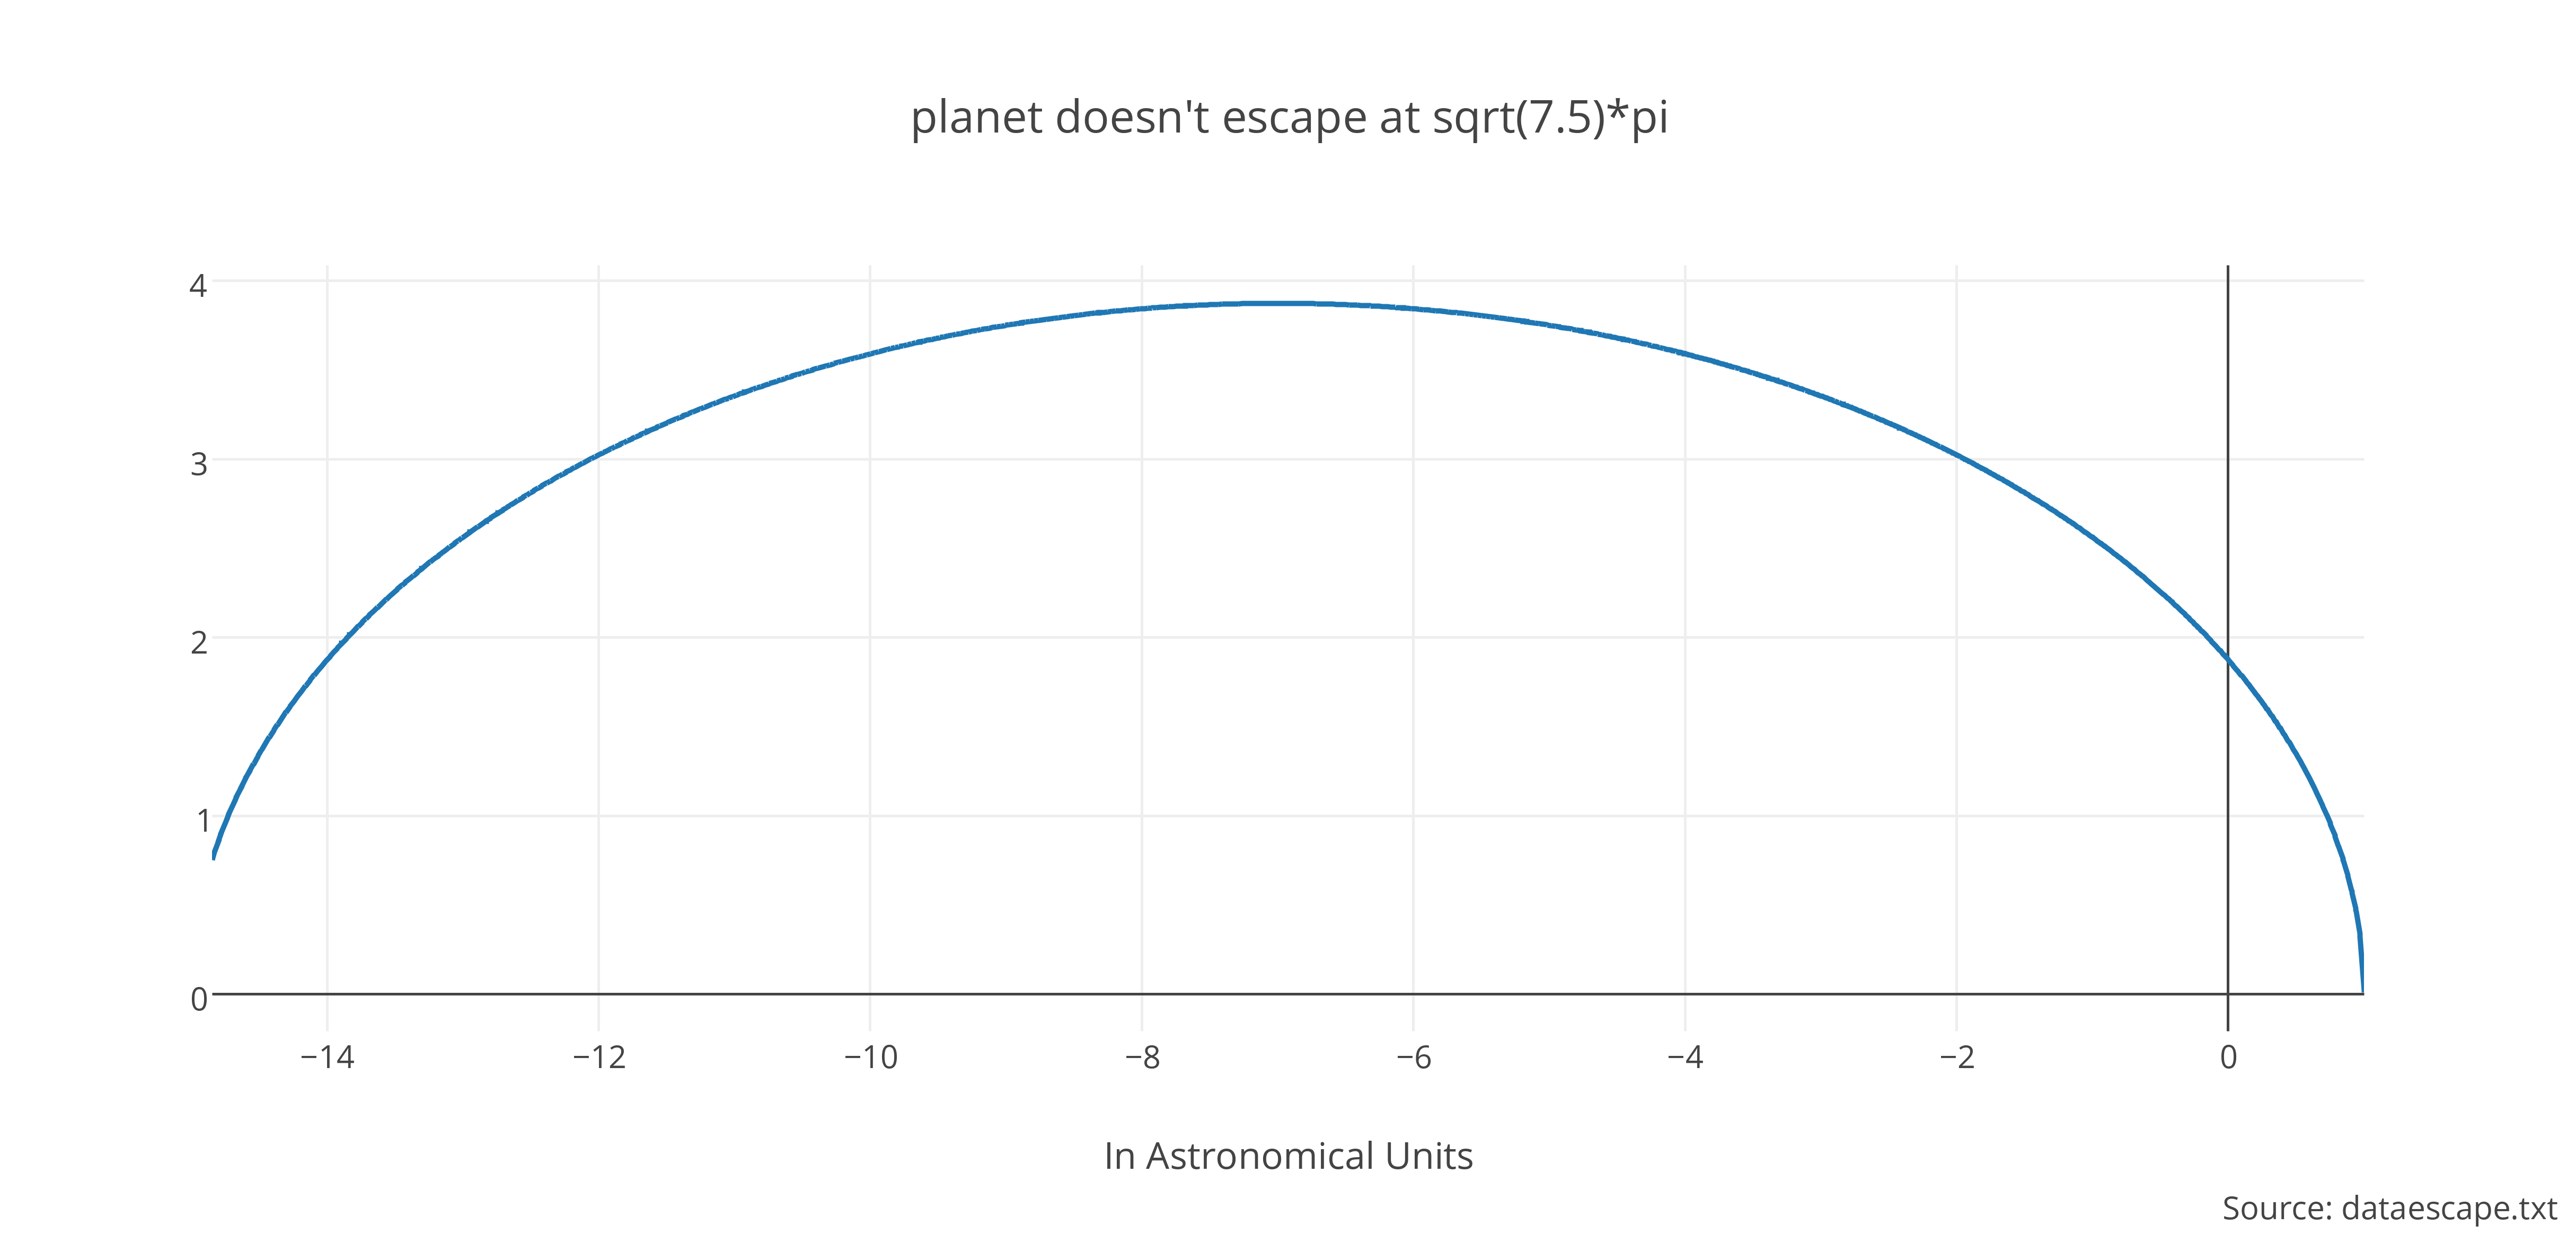
\includegraphics[width=6in]{planet_doesnt_escape_at_sqrt75pi.png}\\

\item[\bf Three-Body Problem ]
Now I add Jupiter to the solar system. The introduction of a third body means that the force interaction between Earth and Jupiter must be accounted for in my code as well as the major force of each body to the sun:
\[
F_{\mathrm{Earth-Jupiter}}=\frac{GM_{\mathrm{Jupiter}}M_{\mathrm{Earth}}}{r_{\mathrm{Earth-Jupiter}}^2},
\]
To do this, my code contains a double loop that calculates the forces and potential energy between all bodies in the solar system. This is useful for easily adding new celestial objects to the solar system. 
\includegraphics[width=6in]{JES.png}\\
Jupiter is a large object (one thousandth the mass of the sun) and perturbs the orbit of the earth. The RK4 and Verlet algorithm is now less stable because of this. I found that when my step length became larger than .05 years, the system would become unstable. Run over long periods of time, one of the positions would diverge, meaning that the object would be ejected out into space. However, keeping the step length at .01 and running the system for 700 years gave pretty stable results. The orbital velocity of Jupiter can be found by the same means as earth's. We can just take a ratio here of the distance from the sun divided by the orbital period. In jupiter's case 5.2AU/12years gives the orbital velocity as .434 that of earth's.  \newline

Now let's examine two cases that can further de-stabilize the solar system. When the mass of Jupiter is increased, this has a noticeable effect on earth. First, when Jupiter is ten times more massive, the solar system is still stable but the earth begins to spiral within its larger orbit around the sun. 
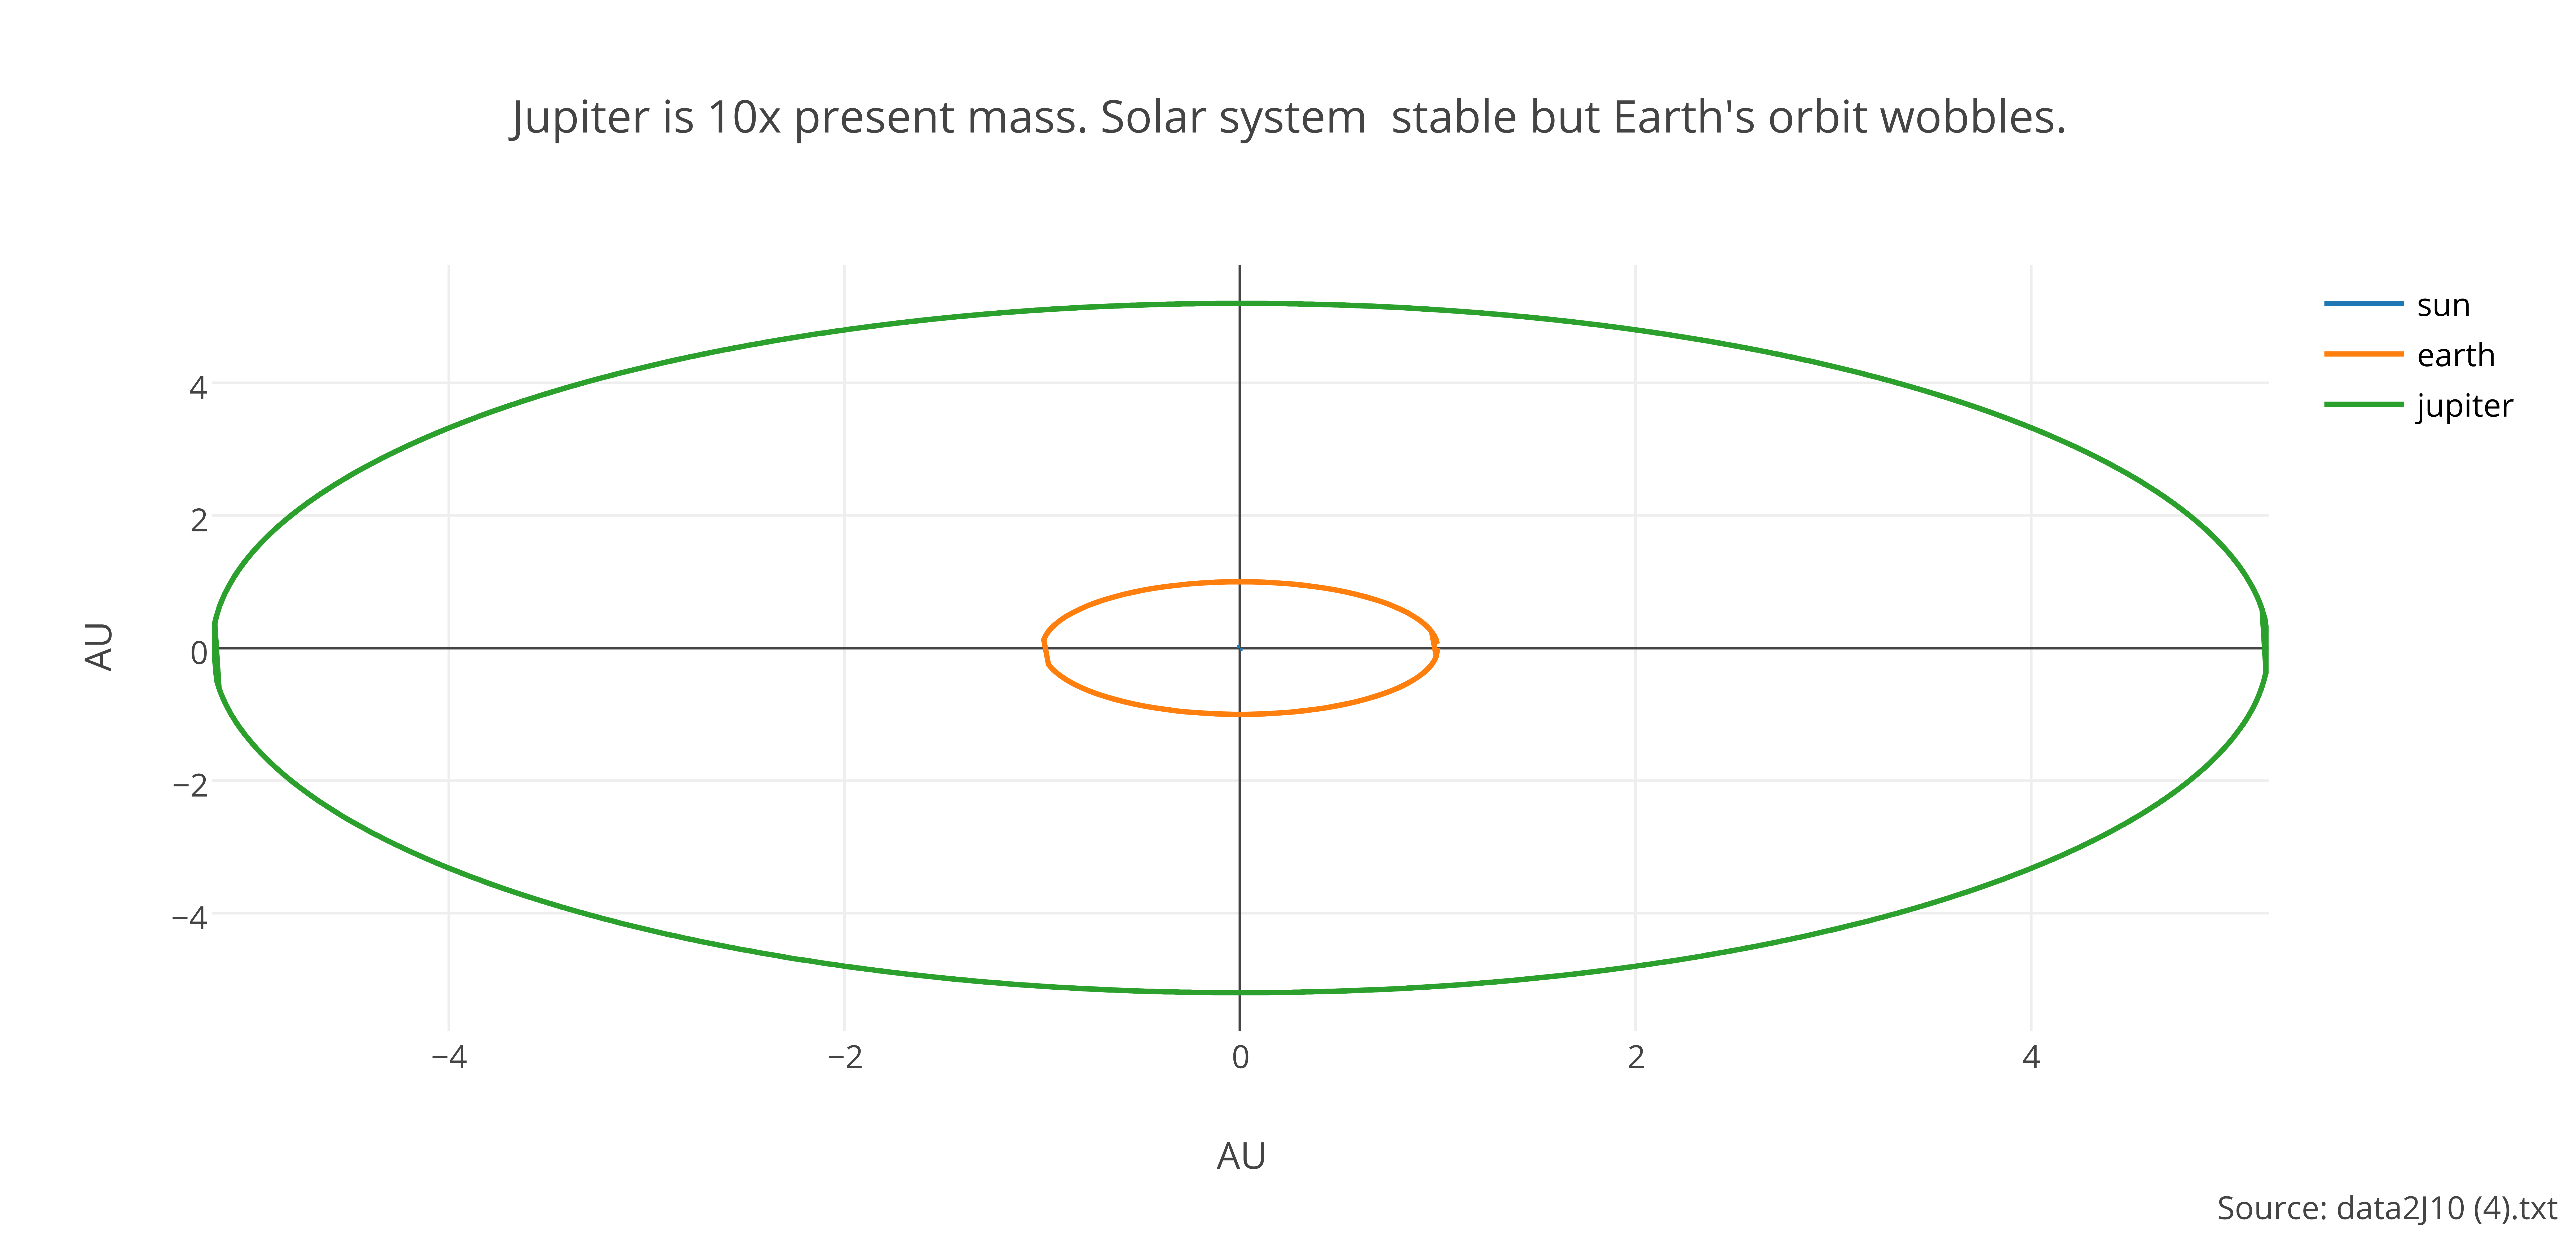
\includegraphics[width=6in]{jupiter_is_10x_present_mass_solar_system_stable_but_earths_orbit_wobbles_.png}\\
When Jupiter is 1000 times more massive then it's equal to the sun. The earth becomes a planet in a binary star system. I'll examine two cases, both of which are unstable for earth and the planet is ejected out from the solar system and a high velocity. In the first graph we see what happens when earth and jupiter start along the same axis although with the earth at 1AU and jupiter at 5.2AU and moving in the same direction. 
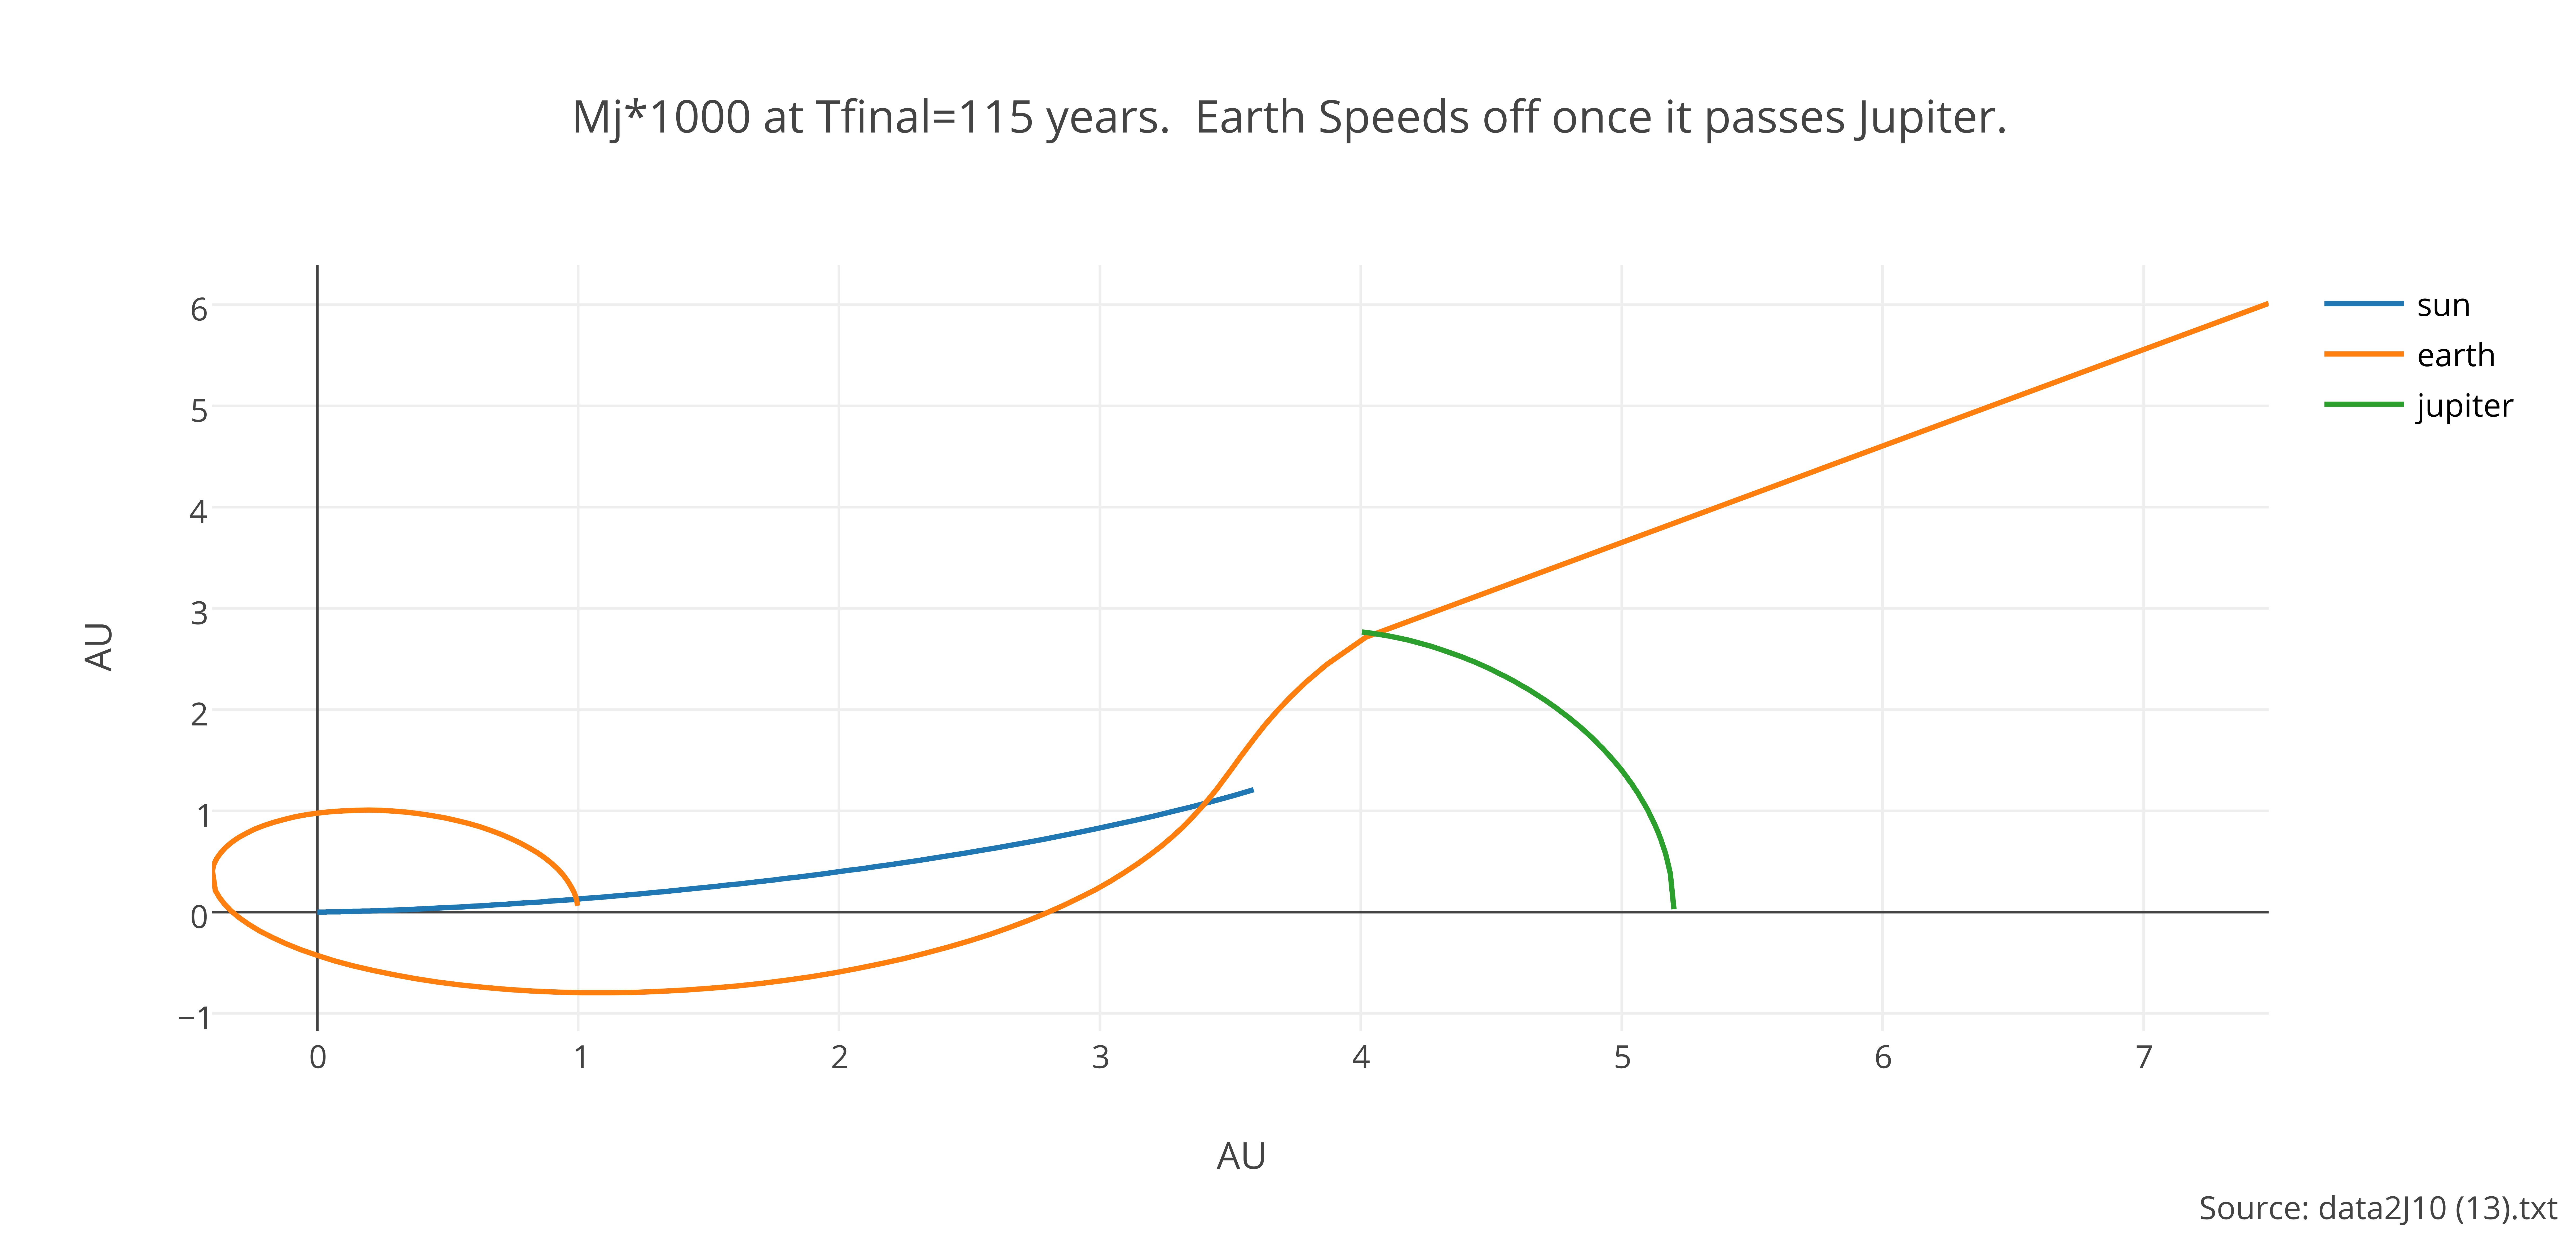
\includegraphics[width=6in]{115yMJ1000.png}\\
The sun and jupiter begin to move toward each other and earth is slingshotted out of the picture. Note, the step length here is .01 years so the timeframe of the motion is 1.15 years. 
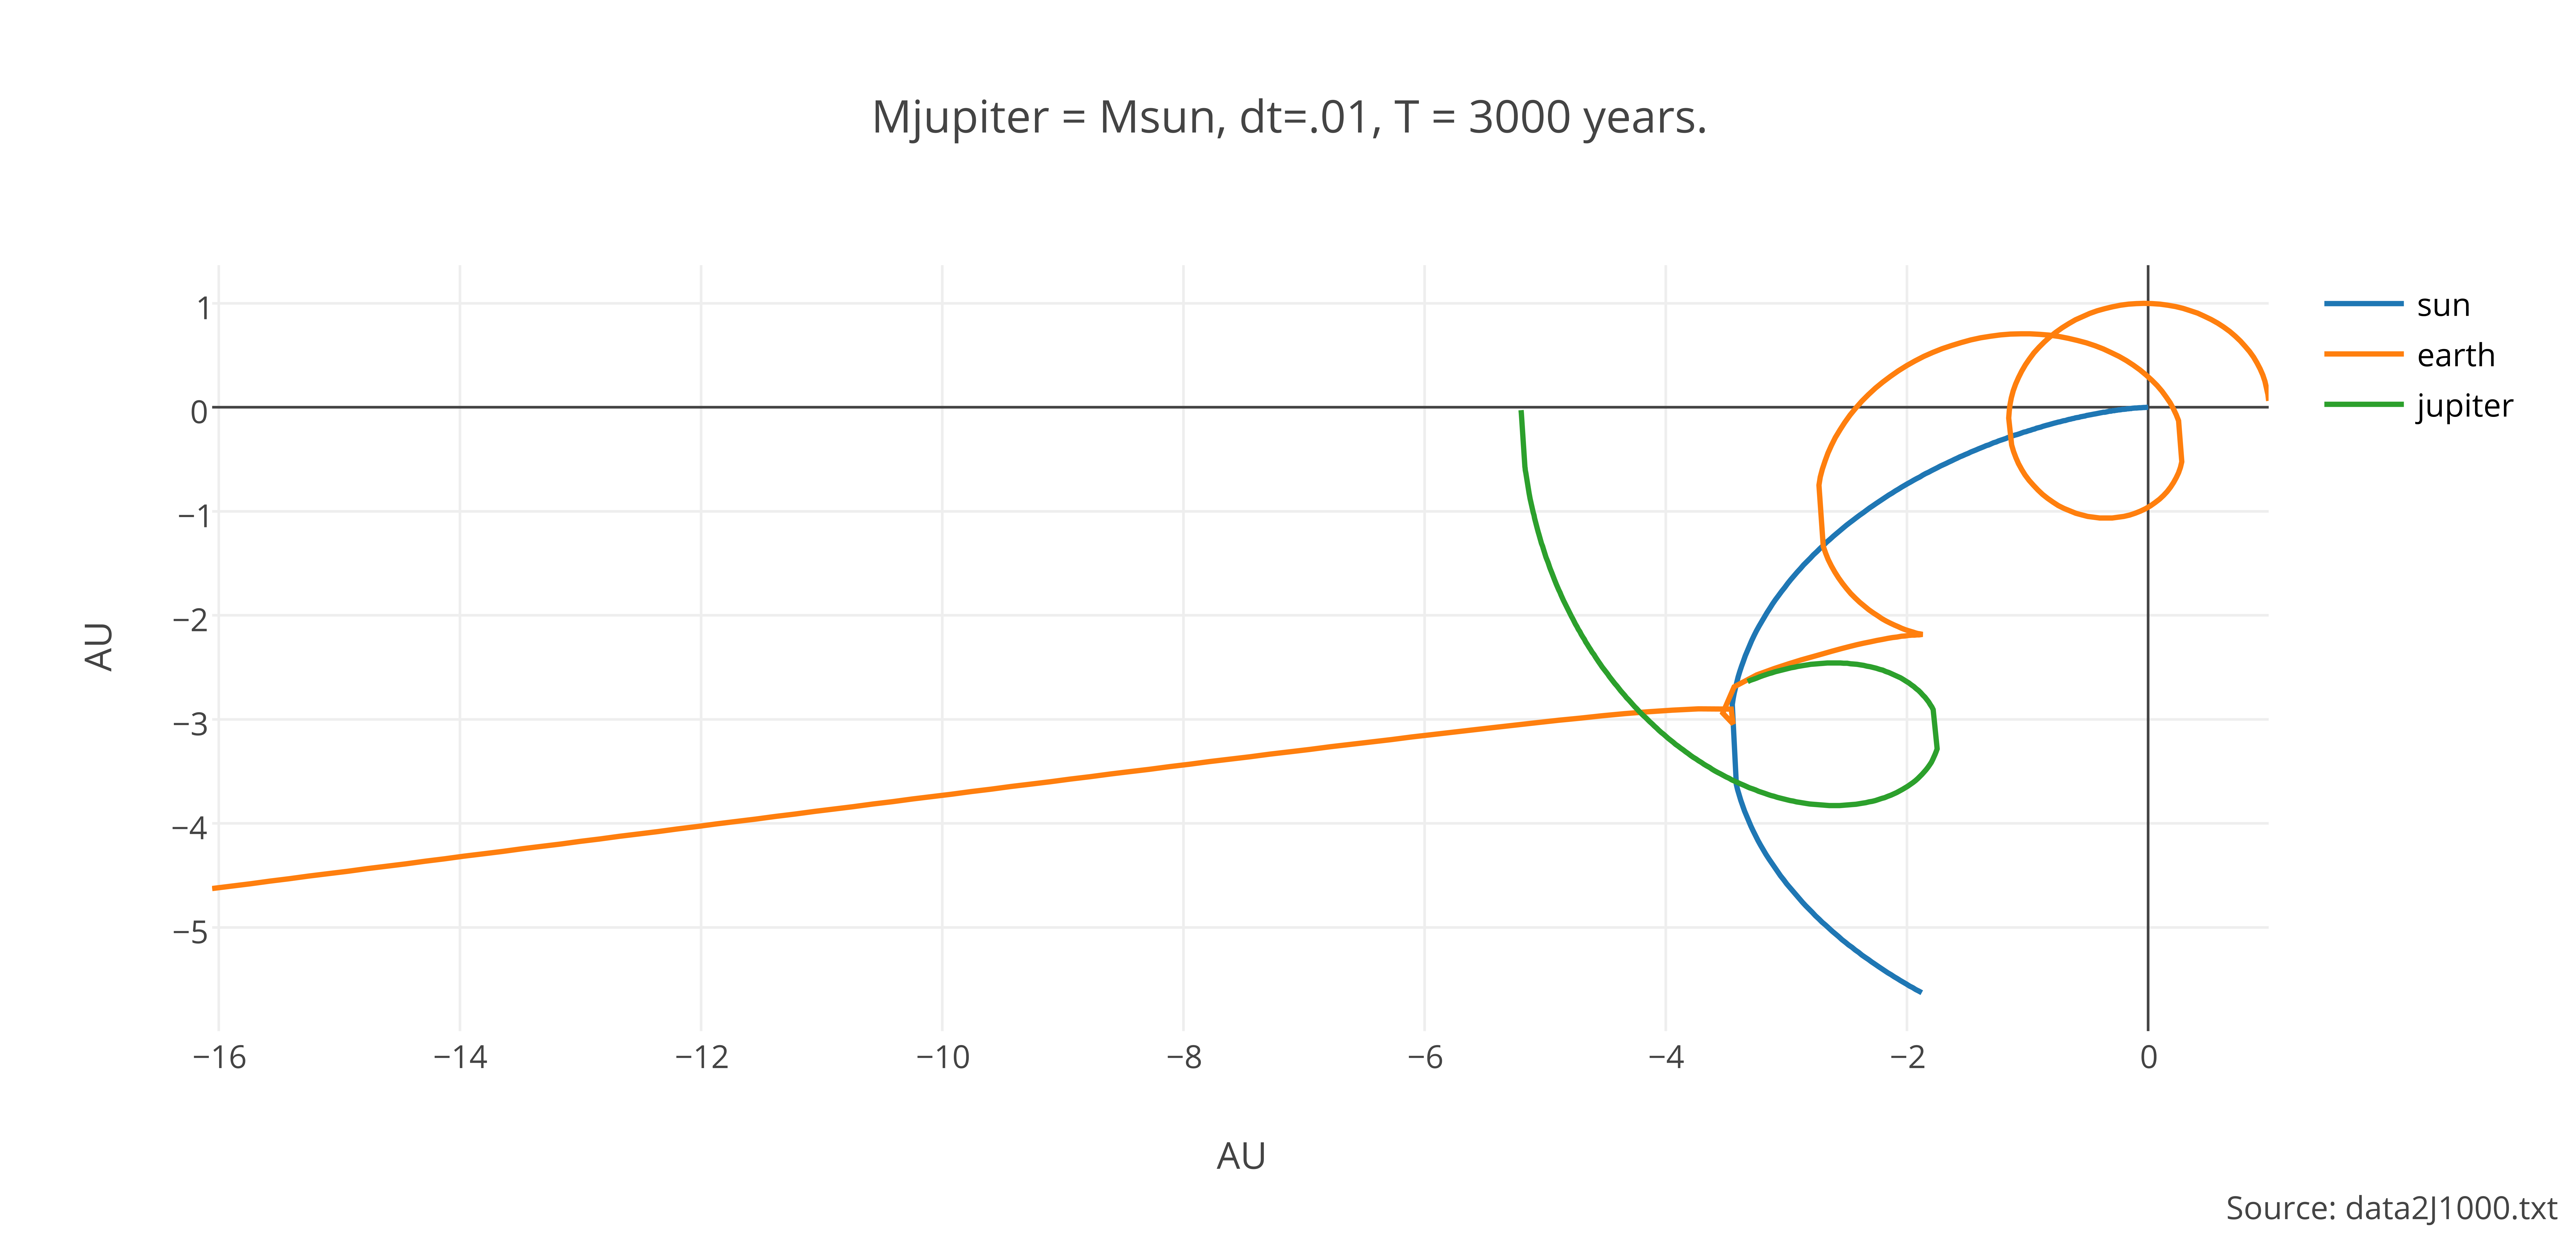
\includegraphics[width=6in]{MJ1000.png}\\
In this graph, earth and jupiter begin along the same axis but this time they move in opposite directions. The step length is again .01 so 30 years are shown. The earth remains in orbit around the binary system for about twice as long in this case but is ultimately ejected. The system is slightly more stable in this case because the momentum imbalance of the system is less severe as compared to the first graph of $M_{jupiter}=M_{\odot}$. \newline
The total momentum of the system needs to be conserved in order for the solar system to be stable. The sun is not stationary but orbits the center of mass of the solar system as do all of the planets. To conserve momentum for the three body simulation, I set the velocity of the sun in such a way that it balances out the momentum contributions from earth and jupiter according to this equation: 
\[
M_{\odot}*vy_{sun}=M_{earth}*vy_{earth} + M_{jupiter}*vy_{jupiter}
\]
We know the velocity of earth is $2*\pi$ and the velocity of jupiter is $.4727*\pi$. Solving for $vy_{sun}$ as all other components are known, we find the sun should have an initial velocity of .00890885 in the opposite direction of the earth's and jupiter's in order to conserve momentum. The results are below.

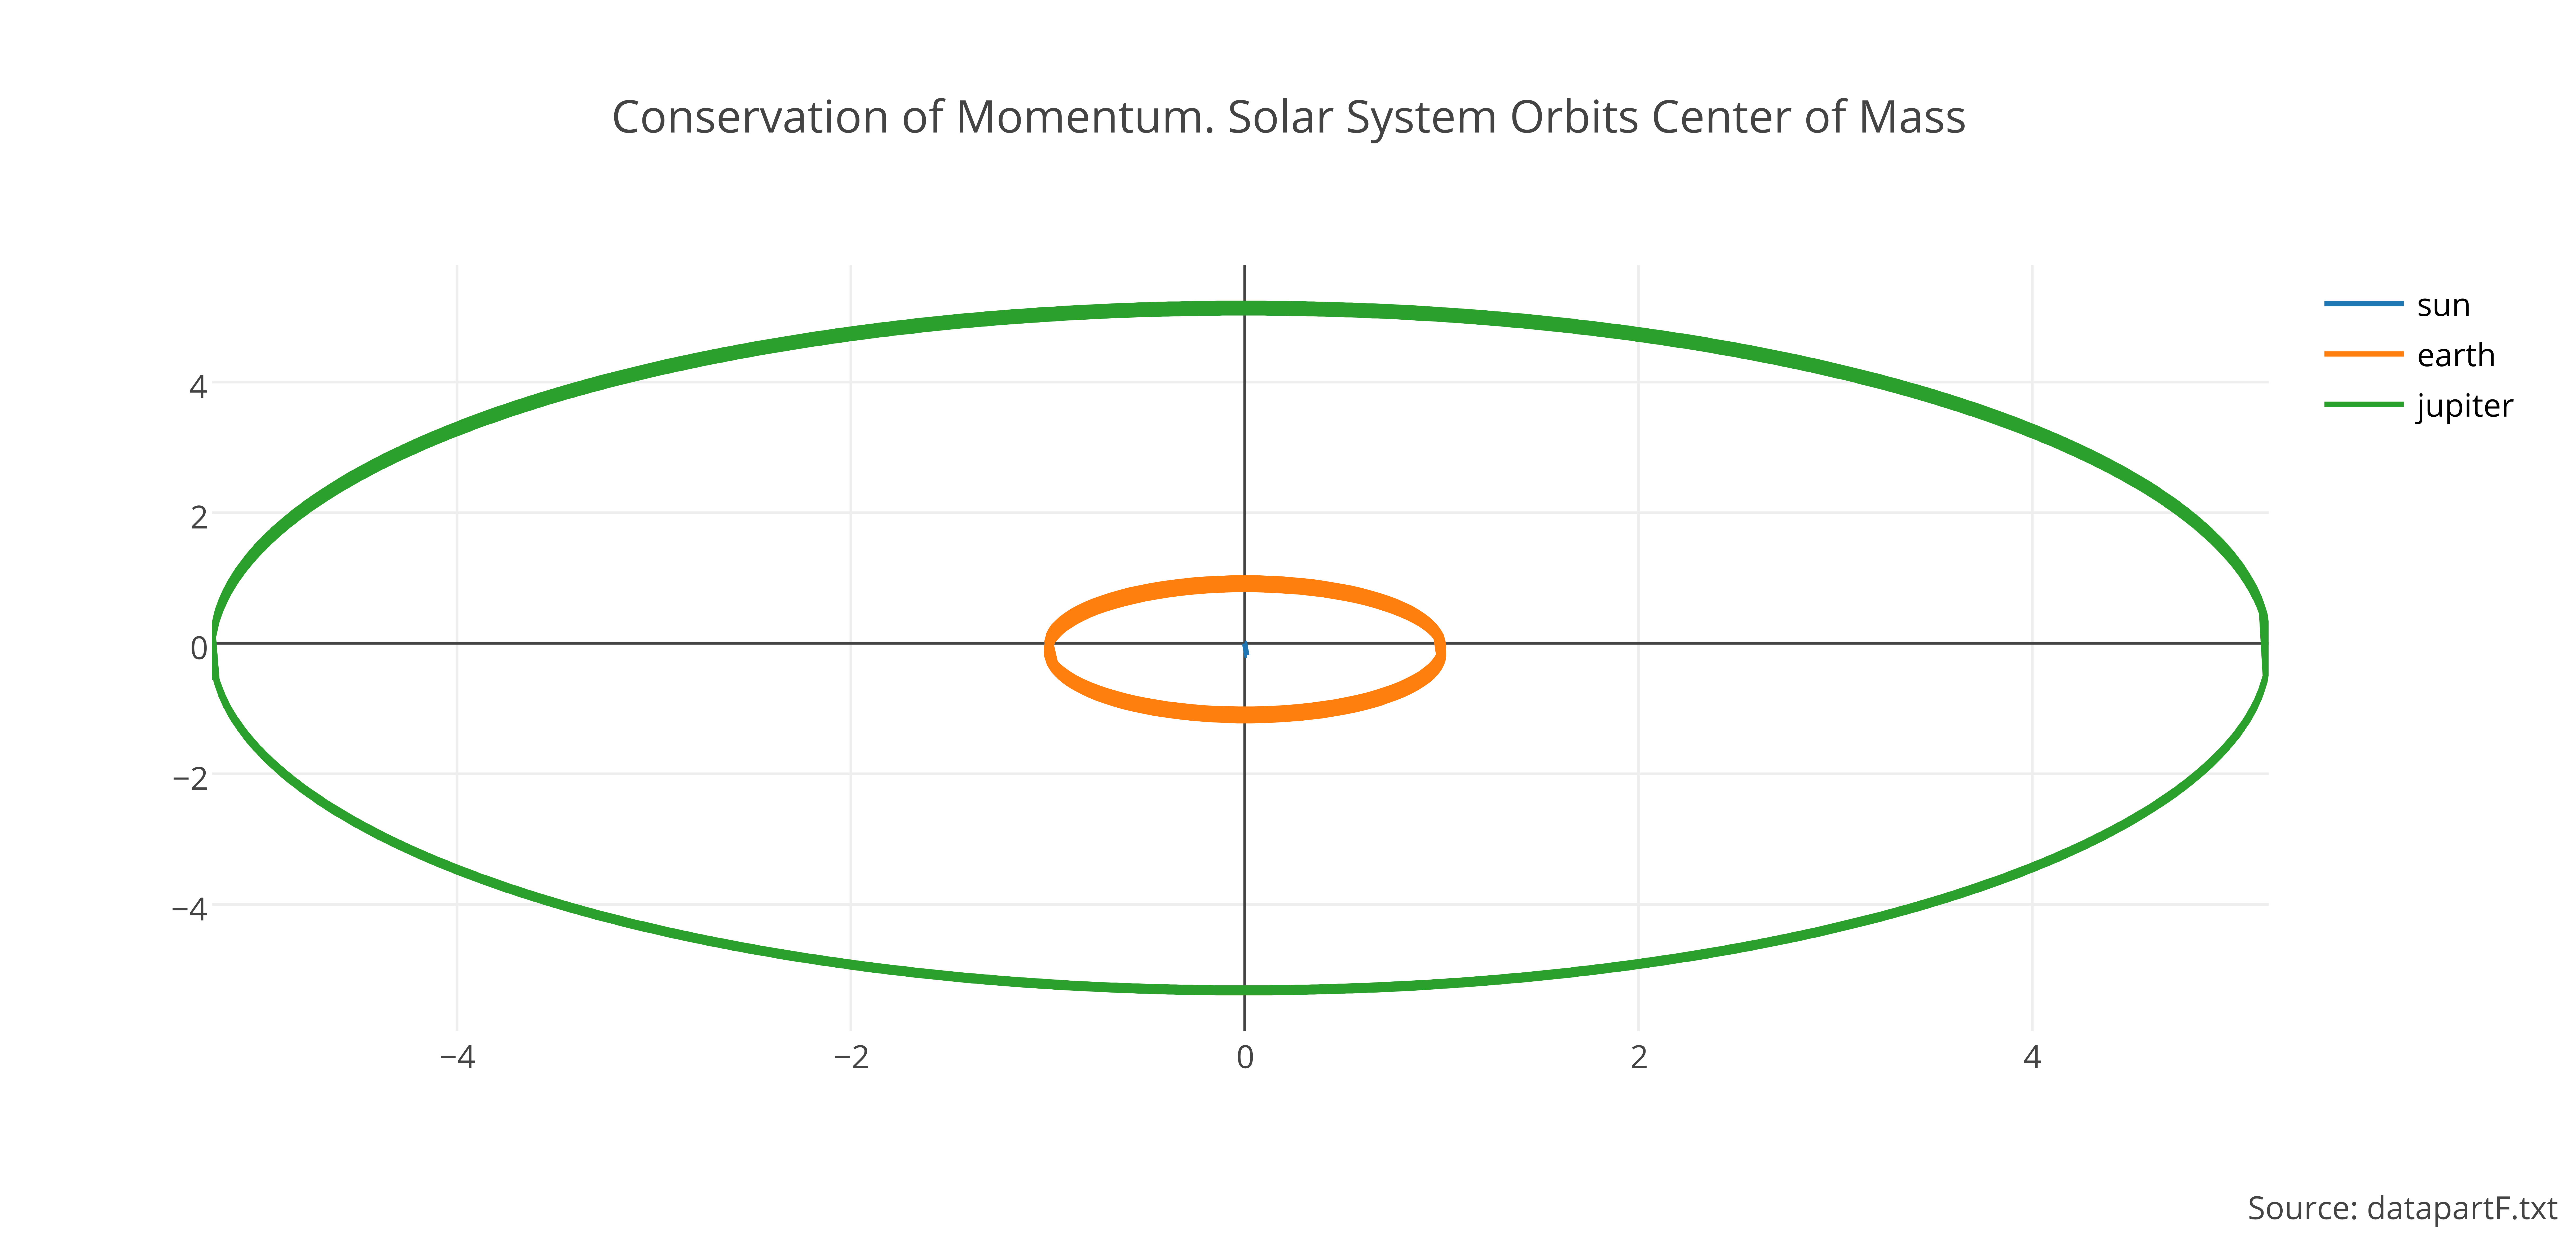
\includegraphics[width=6in]{conservation_of_momentum_solar_system_orbits_center_of_mass.png}\\

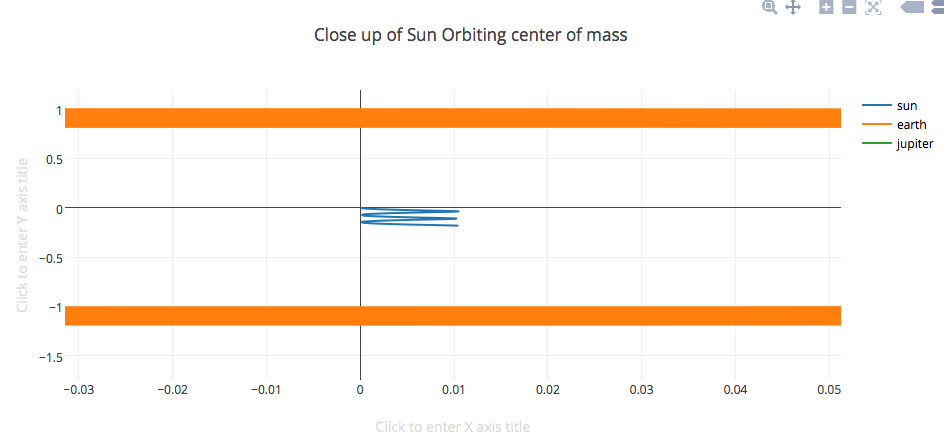
\includegraphics[width=6in]{sunorbit.png}\\
Here we see in the closeup that the sun is not stationary but undulates with the periodicity of the two other smaller bodies. \newline
Finally, I add in all the other planets of the solar system and attempt to keep momentum conserved by calculating the initial velocity based on distance from sun, orbital period, and mass as seen in the following table: 
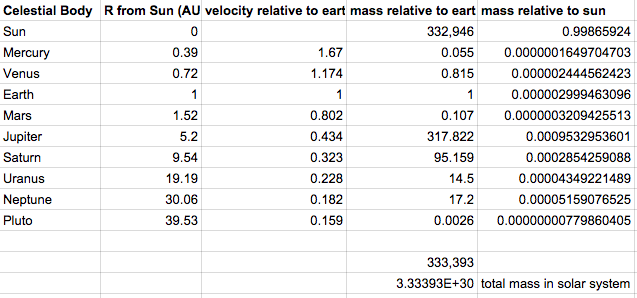
\includegraphics[width=6in]{table.png}\\
The sun's initial velocity was (slightly) increased to accommodate the added planets. The results of the inner planets are included here. The period of observation is 10 years. 
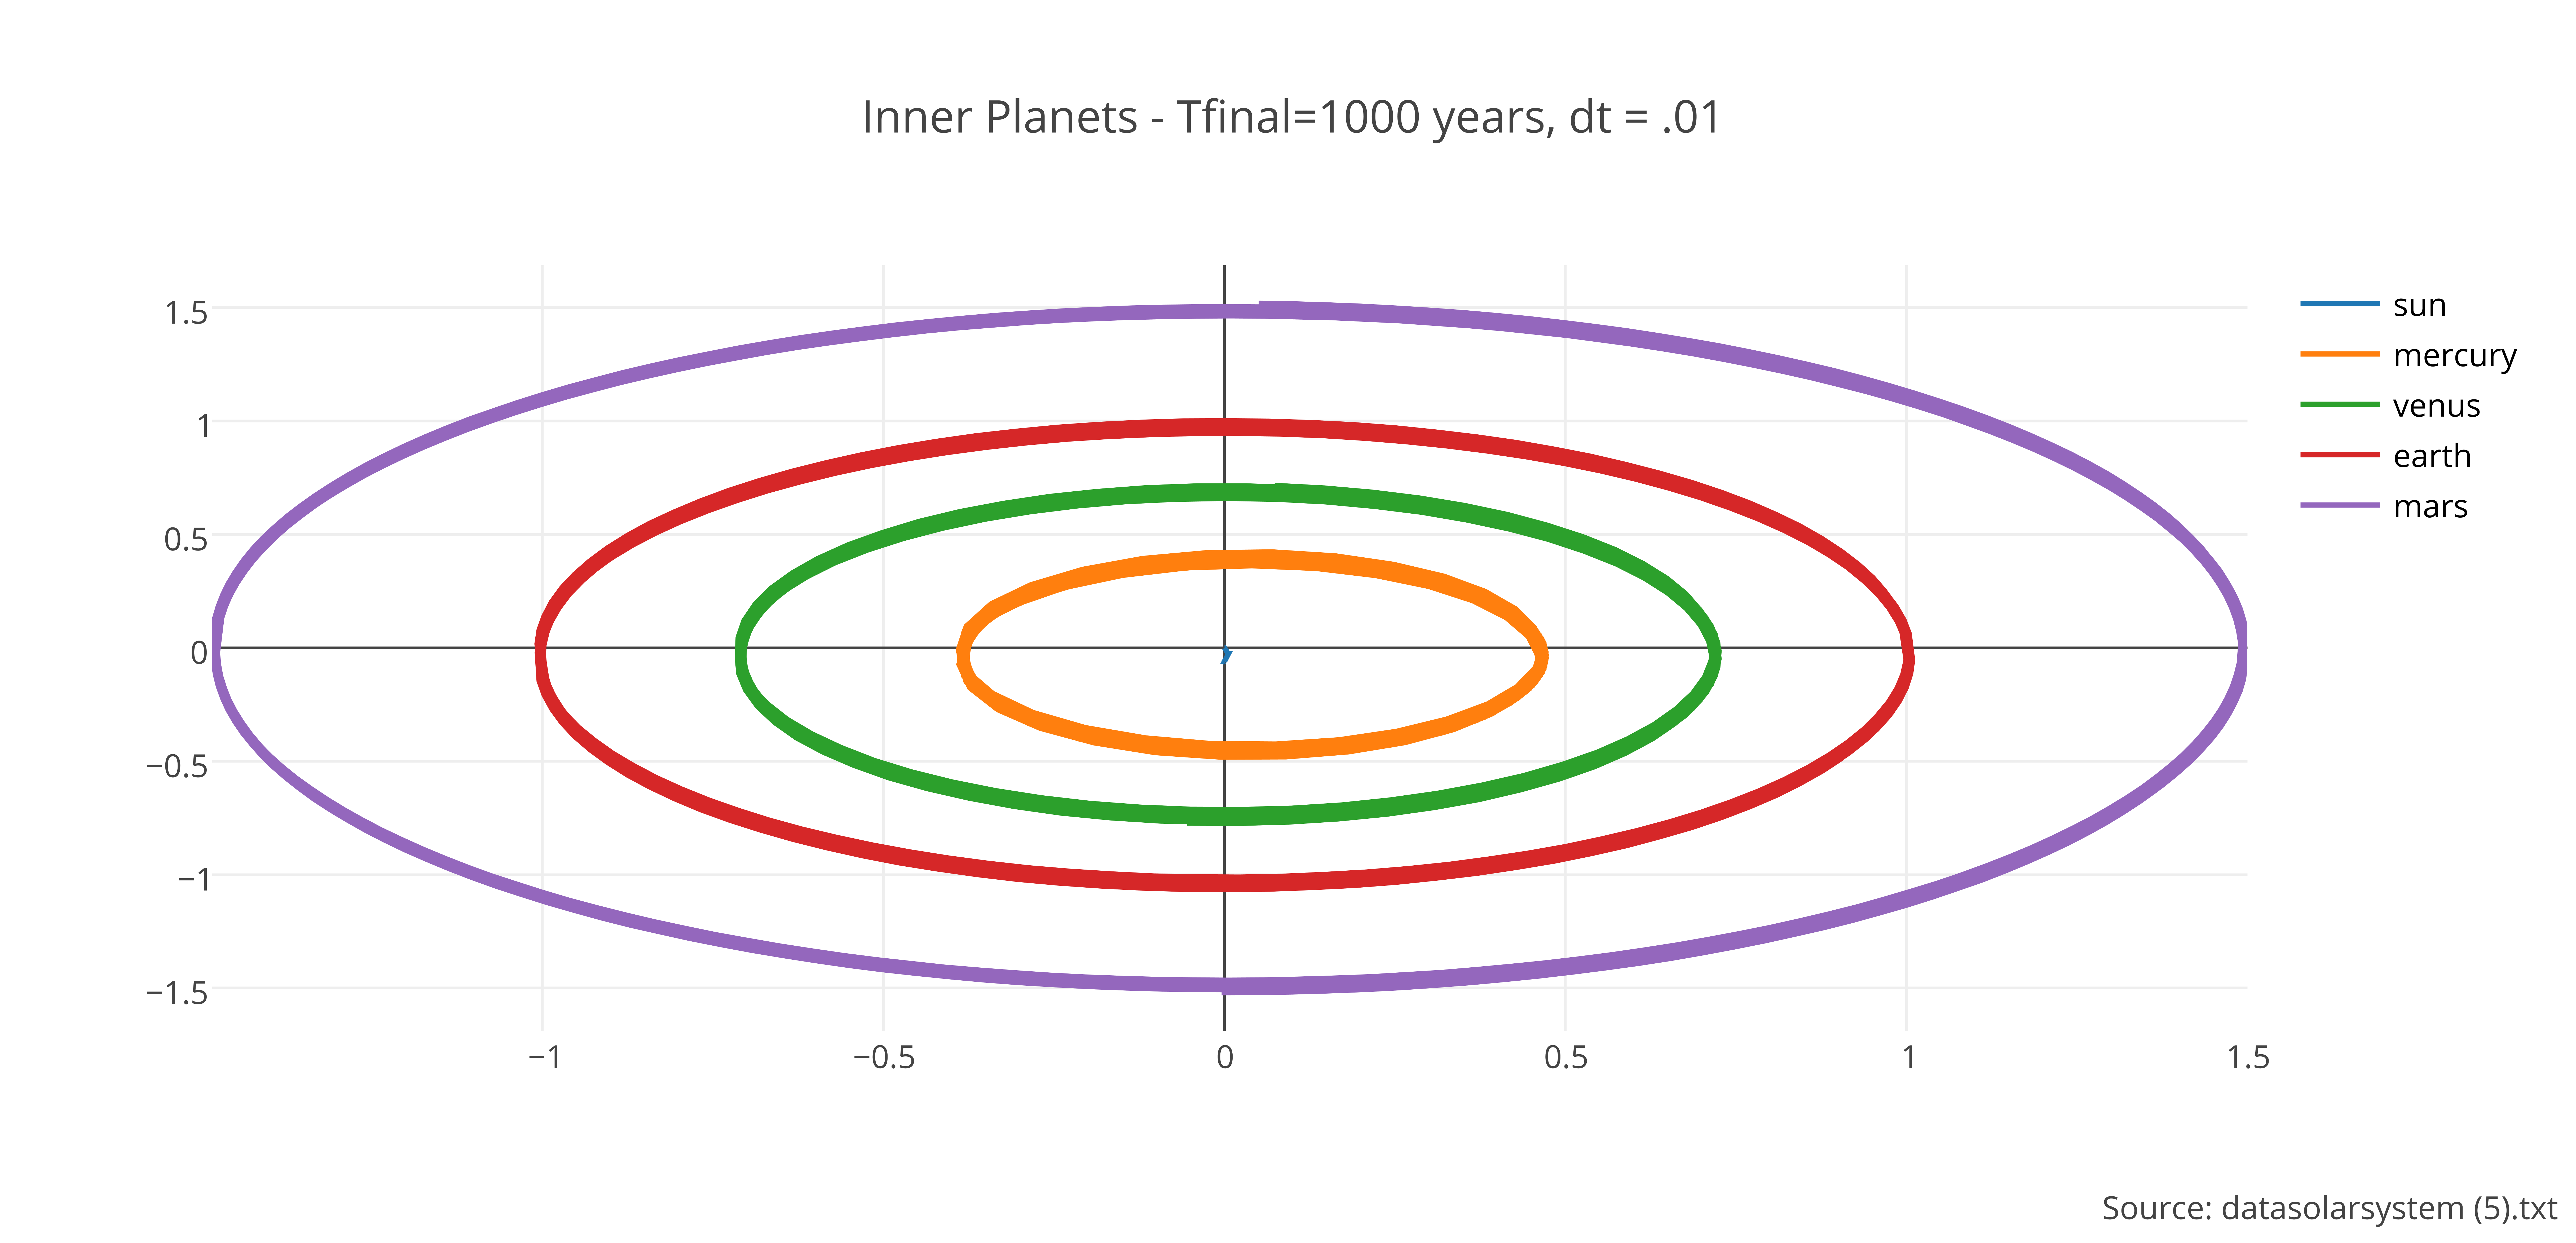
\includegraphics[width=6in]{innerplanets.png}\\
And here is a graph of all the planets, although only the outer orbits are discernible. 
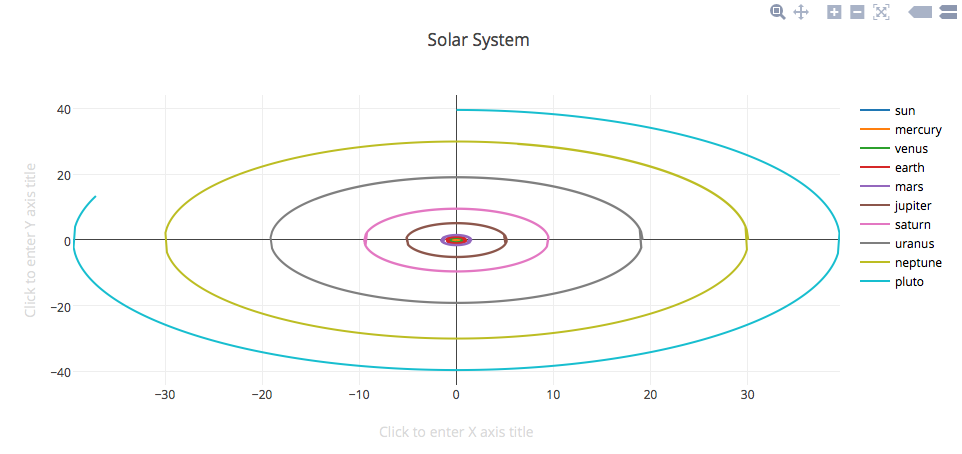
\includegraphics[width=6in]{allplanets.png}\\

The initial positions are arbitrarily estimated as I could not find accurate 2-D cartesian starting points for a circular simulation such as this. Thus, the solar system drifts over a long period of time as seen in this graph. 
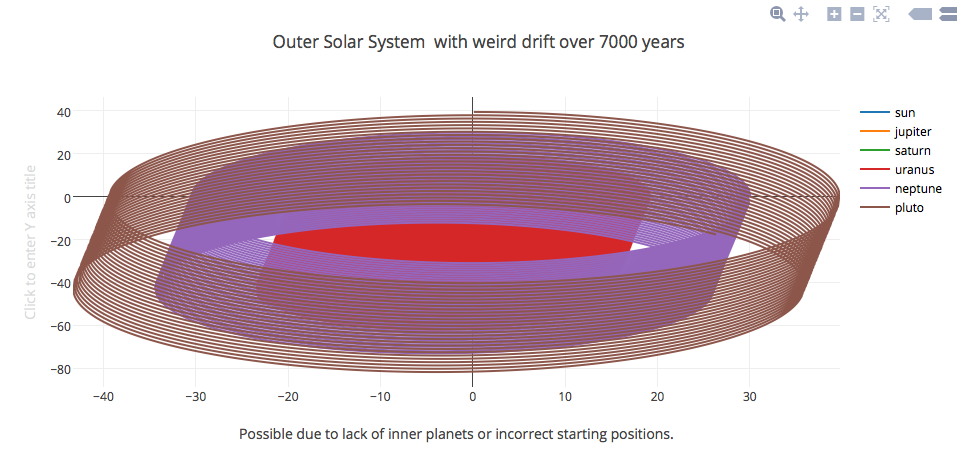
\includegraphics[width=6in]{drift.png}\\



\item[\bf Conclusion]

This project has interesting physical takeaways and demonstrates how some simple algorithms can aid a great deal toward solving problems where there is no easy analytical solution. 

\end{enumerate}


\end{document}

